\chapter{Conclusion: The Invariant Continuum and Falsifiability}
\label{chap:part3_conclusion}

\section{The Kinematic Governing Equations of the Spacetime Gravitational Floor (SGF)}
As rigorously derived throughout Part III and summarized in the \hyperref[app:consolidated_equations]{Consolidated Equations} appendix, the macroscopic behavior of the universe is governed entirely by the native visco-elastic parameters of the Spacetime Gravitational Floor. Tension Field Theory formally replaces the kinematically expanding Friedmann-Lemaître-Robertson-Walker (FLRW) standard model with five exact mechanical state equations.

\vspace{0.3cm}
\noindent \textbf{1. The Visco-Elastic Drag Equation (Replacing Metric Expansion):}
\begin{equation}
    1+z = e^{\frac{\Gamma_D x}{c_E}}
\end{equation}
\textit{Mechanical Translation:} Cosmic redshift is not the stretching of empty space. It is the strict thermodynamic energy dissipation of a transverse wave performing continuous work against the fundamental boundary friction ($\Gamma_D$) of the active lattice.

\vspace{0.3cm}
\noindent \textbf{2. The Non-Linear Redshift Approximation (Replacing Dark Energy):}
\begin{equation}
    d_L = \frac{c_E}{H_0} (1+z)\ln(1+z)
\end{equation}
\textit{Mechanical Translation:} The universe is not accelerating outward. The observational signature attributed to "Dark Energy" is simply the positive second-order term ($+\frac{z^2}{2}$) of the natural logarithmic attenuation curve as lattice drag compounds over extreme cosmic distances.

\vspace{0.3cm}
\noindent \textbf{3. The Kinematic State Equation (Replacing the Friedmann Equation):}
\begin{equation}
    \Gamma_D^2 = \frac{4\pi G}{3} \rho_c
\end{equation}
\textit{Mechanical Translation:} The critical density of the universe is not balancing a kinematic explosion. It is the strict static requirement for phase equilibrium, where the bulk restorative tension of macroscopic gravity ($G\rho_c$) perfectly counterbalances the visco-elastic decay rate of the lattice ($\Gamma_D$).

\vspace{0.3cm}
\noindent \textbf{4. The Causal Mass Limit (Replacing the Infinite Singularity):}
\begin{equation}
    M_U = \frac{c_E^3}{G \Gamma_D}
\end{equation}
\textit{Mechanical Translation:} The universe did not originate from, nor can it collapse into, a point of infinite density. This equation defines the absolute mechanical saturation limit; if mass aggregation attempts to exceed this threshold, the localized holding tension vanishes, triggering catastrophic decompression rather than infinite singularity.

\vspace{0.3cm}
\noindent \textbf{5. The Global Phase Avalanche Equation (Replacing the Linear Age of the Universe):}
\begin{equation}
    M_p(t) = M_{D,G} \cdot e^{\Gamma_D t}
\end{equation}
\textit{Mechanical Translation:} Time is not measured from a geometric genesis. The macroscopic timeline of the universe is a finite thermodynamic clock, strictly governed by the exponential accumulation of topological defects (Black Holes) driven by the universal friction parameter ($\Gamma_D$). This clock ticks inevitably toward the 5.16\% global percolation limit, forcing the cyclical renewal of the cosmos.


\section{Empirical Falsification Criteria}
Tension Field Theory makes the following definitive, testable predictions that directly contradict standard $\Lambda$CDM expectations:

\begin{itemize}
    \item \textbf{Prediction 1: Visco-Elastic Dispersion and the Topological Tail (Falsifying Metric Expansion).} Standard cosmology posits that cosmological time dilation is driven by the uniform stretching of the metric, dictating that a propagating wave packet will stretch symmetrically. Tension Field Theory dictates that time dilation is the structural relaxation of a photon conserving its topology ($N$) against the visco-elastic friction of the SGF. Because this boundary friction is a physical hydrodynamic interaction, we strictly predict that high-resolution temporal integration of isolated, high-redshift transients (e.g., Fast Radio Bursts) will reveal an asymmetric visco-elastic dispersion tail. The wave packet will not stretch uniformly; the leading edge will exhibit a different localized strain profile than the trailing edge. Detecting this asymmetric structural deformation physically proves the wave is plowing through a dissipative medium, definitively falsifying the uniform kinematic expansion of empty space.
    
    \item \textbf{Prediction 2: Mature High-Redshift Galaxies (The JWST Anomaly).} In standard cosmology, high redshift ($z$) corresponds to the ``early universe,'' necessitating that galaxies at extreme distances must be infantile and possess low metallicity. Because TFT proves redshift is an optical distance artifact rather than a temporal epoch, we strictly predict that the James Webb Space Telescope (JWST) will continue to discover massive, fully formed, high-metallicity galaxies at extreme redshifts, physically violating the temporal expansion limits of $\Lambda$CDM.
    
    \item \textbf{Prediction 3: The Constancy of the Local Hubble Drag.} Because the Hubble parameter ($H_0$) is a constant damping rate ($\Gamma_D$) of the visco-elastic lattice, local distance ladder measurements will consistently converge on $\approx 73 \text{ km/s/Mpc}$, irrespective of future instrument calibration. The $67.4 \text{ km/s/Mpc}$ CMB value is a permanent artifact of misapplying a frictionless kinematic acoustic horizon to a physically damped structural boundary.
\end{itemize}

\vspace{0.3cm}

\section{The Phenomenological Translation of Observational Cosmology}

To bridge the phenomenological gap between standard geometric cosmology and solid-state visco-elastic mechanics, Table \ref{tab:cosmic_translation} provides a direct diagnostic translation of the macroscopic observable universe.

\vspace{0.4cm}

\bgroup
\renewcommand{\arraystretch}{1.5}
\small
\setlength{\LTcapwidth}{\textwidth} % <--- THIS COMMAND FIXES THE FOLD
\begin{longtable}{@{} p{3.0cm} p{5.5cm} p{6.5cm} @{}}
\caption{The Phenomenological Translation of Observational Cosmology}
\label{tab:cosmic_translation} \\
\toprule
\textbf{Observational Phenomenon} & \textbf{Standard Cosmology ($\Lambda$CDM) Interpretation} & \textbf{Tension Field Theory (TFT) Mechanical Resolution} \\
\midrule
\endfirsthead

\multicolumn{3}{c}{\textit{Table \thetable\ continued from previous page}} \\
\toprule
\textbf{Observational Phenomenon} & \textbf{Standard Cosmology ($\Lambda$CDM) Interpretation} & \textbf{Tension Field Theory (TFT) Mechanical Resolution} \\
\midrule
\endhead

\bottomrule
\endfoot

\textbf{Cosmic Expansion} & Literal expansion of ``empty space'' with no physical substance or cause. & \textbf{Eliminated.} The lattice is statically bounded. Expansion is an optical illusion caused by the kinematic drag ($H_0$) of the SGF. \\
\textbf{The Hubble Law} & Interpreted as a kinematic Doppler shift (galaxies receding). & \textbf{Re-interpreted.} Redshift is the visco-elastic energy dissipation of transverse waves passing through the dual phase vacuum. \\
\textbf{Cosmic Age ($13.8 \text{ Byr}$)} & The temporal age of the universe originating from a singularity. & \textbf{Re-interpreted.} It is the fundamental visco-elastic decay time—recalibrated to $13.39 \text{ Byr}$ based on local SGF drag. It represents the characteristic $e$-folding time required for lattice friction to drain $63.2\%$ of an optical wave's kinematic energy, beyond which distant structures geometrically fade into the thermal background. \\
\textbf{Critical Density ($\rho_c$)} & An arbitrary geometric threshold defining metric flatness. & \textbf{Mechanically Defined.} It is exactly the structural defect capacity ($\alpha_G=1$) required to locally saturate the SGF lattice ($\Gamma_D^2 = \frac{4\pi G}{3} \rho_c$). \\
\textbf{CMB} & Leftover flash of the primordial Big Bang (Recombination Epoch). & \textbf{Active State.} It is the active, isotropic thermal exhaust of transverse light waves continuously degrading into longitudinal lattice vibrations (phonons). \\
\textbf{BAO Anisotropies ($1.04^\circ$)} & A temporal snapshot of primordial quantum/acoustic fluctuations. & \textbf{Structural Shadow.} The permanent thermodynamic silhouette of the $\approx 42.75 \text{ Mpc}$ macroscopic density rings located at the Viscous Cosmic Horizon. \\
\textbf{Black Holes \& The Cosmos} & Treated as entirely separate metric phenomena. & \textbf{Unified.} The total observable cosmos operates at the exact mechanical saturation limit of a Type I Black Hole ($M_U = M_{\text{Sat}}$). \\
\textbf{Type Ia Supernovae} & Appear too dim; interpreted as proof that metric expansion is accelerating. & \textbf{Optical Friction.} Natively resolved by the $+z^2/2$ Taylor expansion of exponential lattice drag. No acceleration exists. \\
\textbf{Dark Energy ($\Lambda$)} & An ad hoc, un-sourced vacuum energy ($w=-1$) forcing metric acceleration. & \textbf{Eliminated.} The mathematical ghost of visco-elastic optical drag (the $+z^2/2$ Taylor expansion) compounding over extreme distances. \\
\end{longtable}
\egroup

\section{Kinematic Capacity and The Invariant Continuum}

Physics must re-examine the foundational assumption of an empty geometric void. The universe is not an infinitely expanding geometry leading to thermodynamic failure; it is a spatially bounded, perpetual macro-mechanical oscillator driven by strict thermodynamic phase cycles.

The operational limits of causality within this universe are dictated entirely by a single structural relationship: The Kinematic Capacity vs. The Strain Load.

\begin{itemize}
    \item \textbf{The Capacity ($c_E^2$):} The absolute kinematic energy budget of a single Face-Centered Cubic (FCC) lattice node.
    \item \textbf{The Load ($\alpha_G$):} The universal strain gauge measuring how that kinematic capacity is consumed.
\end{itemize}

Whenever the local strain load strictly equals the capacity ($\alpha_G=1$), the active vacuum undergoes causal failure. Tension Field Theory unites the absolute extremes of existence by proving that this exact same mechanical threshold ($\alpha_G=1$) manifests in three distinct modes of causal limits:

\subsection{Type I: Gravitational Causal Failure (The Black Hole)}
\begin{itemize}
    \item \textbf{Mechanism:} Inertial Saturation (The Density Limit).
    \item \textbf{Physics:} When mass is severely concentrated at the microscopic scale ($10^{-26} \text{ m}$), the local strain load exhausts the $c_E^2$ capacity of the node. Reaching a trigger density of $\approx 10^{70} \text{ kg/m}^3$, the node mechanically snaps, losing its shear elasticity and locking into the Simple Cubic (SC) geometry.
    \item \textbf{State:} The localized region fully freezes into a zero-void SC sink, achieving a maximum structural density of $\rho_S \approx 10^{96} \text{ kg/m}^3$. Because the core has no voids, the effective inertia diverges ($\mu_{\text{eff}} = \mu_D (1-\alpha_G)^{-4}$), and transverse light propagation ($c_P$) strictly ceases. The massive topological strain (inertial mass) is mechanically displaced by the advancing crystallization front, segregating strictly onto the singular boundary layer (the Event Horizon).
\end{itemize}

\subsection{Type II: Cosmological Causal Saturation (The Viscous Cosmic Horizon)}
\begin{itemize}
    \item \textbf{Mechanism:} Cumulative Drag (Distance/Energy Exhaustion).
    \item \textbf{Physics:} When mass is naturally distributed to the critical density ($\rho_c$), the structural load is gradually integrated over a vast macroscopic distance. At the local causal radius ($R_U \approx 10^{26} \text{ m}$), the cumulative gravitational potential ($\int \frac{G \cdot dm}{r}$) exactly equals $c_E^2$.
    \item \textbf{State:} Phase Equilibrium. Because there is no internal structural pressure, the lattice does not break. Instead, propagating transverse waves simply exhaust their kinematic capacity via continuous visco-elastic decay ($E_{\text{obs}} = E_{\text{emit}} e^{-\Gamma_D x / c_E}$), degrading into longitudinal phonons to form the isotropic $2.725 \text{ K}$ Cosmic Microwave Background (CMB) bed. The physical FCC lattice seamlessly survives this optical saturation, tiling outward to form the total Cosmic Reservoir ($R_{\text{Res}} \approx 10^{35} \text{ m}$).
\end{itemize}

\begin{figure}[H]
    \centering
    \includegraphics[width=0.9\textwidth]{Fig23_PartIII_CausalHierarchy.pdf}
    \caption{\textbf{The Causal Hierarchy (Mechanical vs. Energetic Horizons).} 
\textbf{(a) Type I Causal Failure (The Black Hole):} Represents the crystallographic phase lock of the local vacuum. As density reaches the convergence limit ($\rho_{QG}$), the active FCC lattice undergoes a phase transition to the fully packed SC Substrate, eliminating the interstitial voids necessary for vibration. This geometric lock causes the local effective inertia to diverge ($\mu_{\text{eff}} \rightarrow \infty$), making transverse wave propagation mechanically impossible ($c_P = 0$). The light cones squeeze completely shut, irrevocably halting all causal trajectories against the static core. 
\textbf{(b) Type II Causal Saturation (The Viscous Cosmic Horizon):} Represents the thermodynamic energy exhaustion of the wave. The background medium remains structurally intact (FCC), and the macroscopic light cones remain geometrically uniform. However, cumulative visco-elastic drag ($\Gamma_D$) continuously forces the wave into simultaneous vertical compression and longitudinal elongation. This macroscopic friction drives a strict exponential thermodynamic decay of the signal ($E_{\text{obs}}$), fully exhausting the photon's invariant transverse energy budget ($c_E^2$) exactly at $R_U$.}
\label{fig:causal_hierarchy}
\end{figure}

\subsection{Type III: Kinematic Causal Failure (The Nyquist Limit)}
\begin{itemize}
    \item \textbf{Mechanism:} Kinematic Saturation (The Quantum Energy Limit).
    \item \textbf{Physics:} In solid-state mechanics, the Nyquist limit dictates that a transverse wave cannot propagate if its wavelength is physically shorter than the fundamental structural grain of the medium. Setting the minimum wavelength to the active FCC Node Radius ($\lambda_{\mathrm{min}} = r_{\mathrm{D}} \approx 7.89 \times 10^{-27} \text{ m}$) defines the absolute Quantum Energy Limit ($E_{\mathrm{Q}}$) for a single photon:
    $$E_{\mathrm{Q}} = \frac{h c_{\mathrm{E}}}{r_{\mathrm{D}}} \approx 25.18 \text{ J} \approx 1.571 \times 10^{11} \text{ GeV}$$
    \item \textbf{State (The Kinematic Stall):} If a localized event attempts to inject a photon exceeding this limit, the spatial gradient required for linear propagation is destroyed ($v \to 0$). The entire $2\pi$ phase twist is forced into a single node. At this boundary, the geometric strain hits the absolute localized Node Yield Tension ($\tau_{\mathrm{D}} = c_{\mathrm{E}}^4 / G r_{\mathrm{D}}$), and the vacuum ceases to act as a linear spring, becoming highly anharmonic.
    \item \textbf{Resolution (Non-Linear Scattering):} This stalled $25.18 \text{ J}$ is vastly below the $10^{17} \text{ J}$ required to physically shatter the node into a State II black hole, and it lacks the dense nuclear anvil required to coil into stable chiral matter ($e^-, e^+$). Therefore, rather than undergoing a structural phase transition, the lattice violently rejects the anomaly. Acting as a perfect non-linear rigid reflector, the $\tau_{\mathrm{D}}$ boundary forces the stored energy to physically broaden to escape the kinematic stall. The wave is mechanically ripped apart by the surrounding FCC axes, undergoing spontaneous parametric down-conversion as the $25.18 \text{ J}$ scatters into a cascade of lower-energy photons ($\lambda > r_{\mathrm{D}}$) capable of stable spatial propagation. This mechanism structurally forbids the infinite energies and ``ultraviolet catastrophes'' of standard quantum mechanics.
\end{itemize}

\section*{Summary: The Unified Phase Map of the Universe}
\addcontentsline{toc}{section}{\protect\numberline{}Summary: The Unified Phase Map of the Universe}

The macroscopic scale of the observable universe ($\approx 10^{26} \text{ m}$) is not a random evolutionary epoch; it is the strict geometric boundary where the energy of propagating light perfectly balances the visco-elastic drag of the lattice, forming the Viscous Cosmic Horizon.

However, optical exhaustion is not the true end of causality. The absolute thermodynamic expiration of the lattice occurs at the Kinematic Capacity Limit ($L_{\text{max}} \approx 10^{28} \text{ m}$), where the localized accumulation of defect mass reaches global topological percolation ($M_{\text{trg}} \approx 10^{78} \text{ kg}$). Because this absolute chronological expiration occurs vastly earlier than a signal could ever reach the physical Deflation boundary ($R_{\text{rup}} \approx 10^{34} \text{ m}$), the universe contains a massive, permanent Domain of Opaque Causality.

The total Cosmic Reservoir reaches its massive structural span ($R_{\text{Res}} \approx 10^{35} \text{ m}$) not through ongoing kinematic expansion, but as the strict volumetric requirement of the fully decompressed State I FCC lattice. The grand macroscopic boundaries ($10^{26} \text{ m}$, $10^{28} \text{ m}$, and $10^{35} \text{ m}$) and the microscopic quantum depths ($10^{-26} \text{ m}$ and $10^{-35} \text{ m}$) are not governed by disparate regimes. As mapped in Figure \ref{fig:unified_phase_map}, they are dictated by the exact same invariant continuum law of mechanical capacity and visco-elastic load.

\begin{figure}[H]
    \centering
    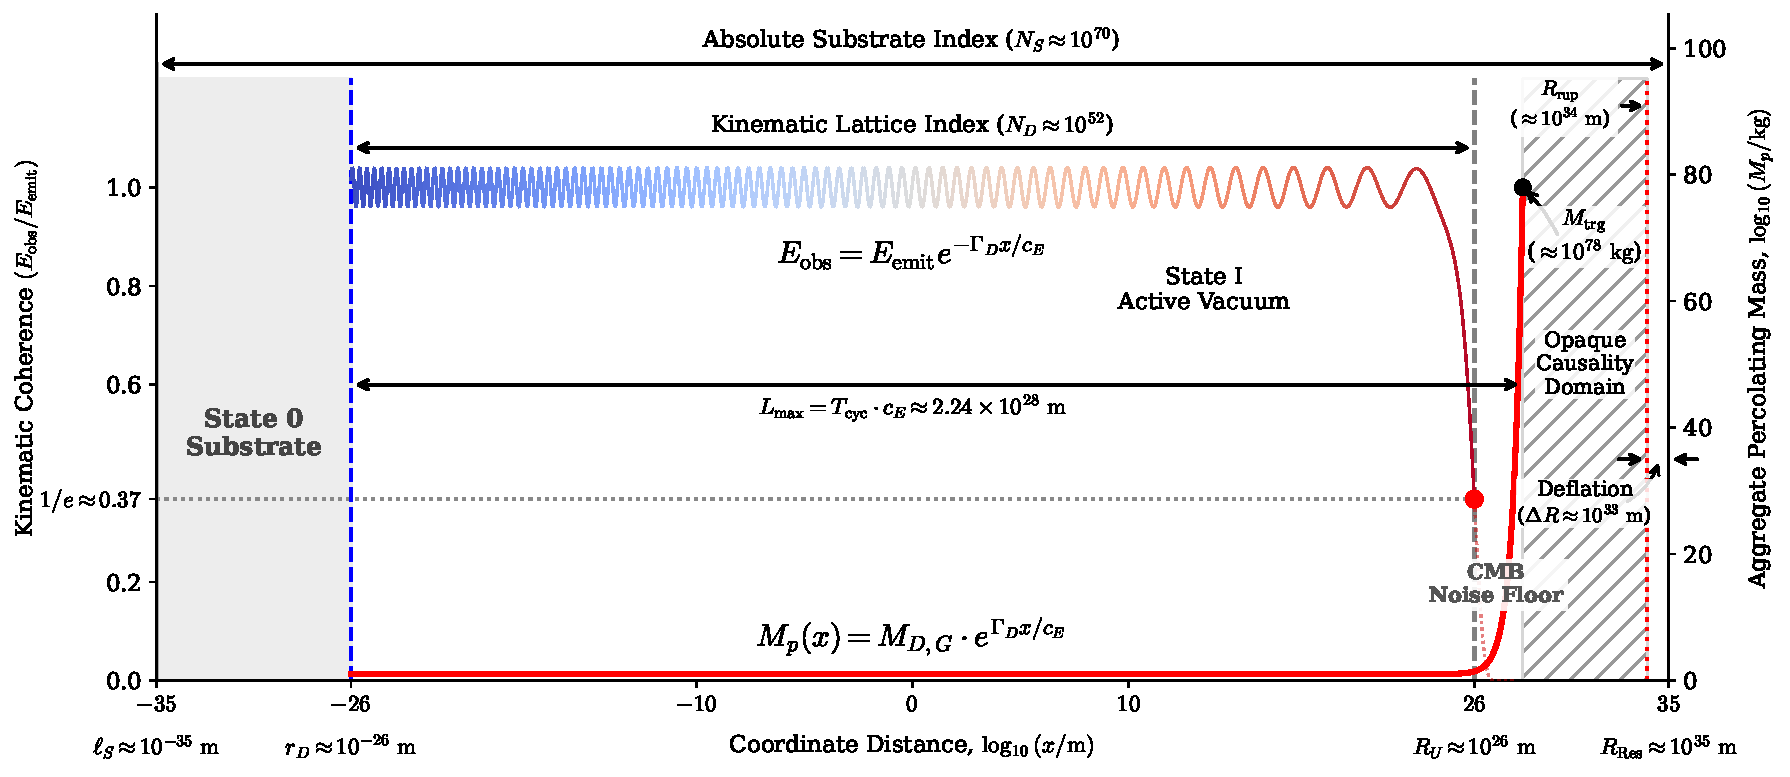
\includegraphics[width=\textwidth]{Figures/Fig24_PartIII_CosmicFinalDiagram.pdf}
    \caption{\textbf{The Unified Phase Map of the Macroscopic Oscillator.} This diagram maps the absolute causal boundaries of Tension Field Theory across 70 orders of magnitude. 
    \textbf{Left (The Wall):} The timeless, rigid Simple Cubic geometry of the State 0 Substrate strictly bounds the active universe at $\ell_S \approx 10^{-35} \text{ m}$. 
    \textbf{Center (The Arena):} Within the vast physical expanse of the State I Active Vacuum, the observable kinematic envelope spans $10^{52}$ orders of magnitude ($N_D$). A transverse wave (blue) degrades due to visco-elastic drag ($e^{-\Gamma_D x/c_E}$), falling to the $1/e$ threshold exactly at the Viscous Cosmic Horizon ($R_U \approx 10^{26} \text{ m}$) where it thermalizes into the CMB. 
    \textbf{Right (The Expiration):} Entirely decoupled from optical decay, the Global Phase Avalanche (red curve) tracks the exponential accumulation of macroscopic defect mass ($M_p$). The thermodynamic clock triggers a vertical asymptote (Critical Divergence), hitting the global percolation threshold ($M_{\text{trg}}$) exactly at the absolute kinematic expiration limit ($L_{\text{max}} \approx 10^{28} \text{ m}$). 
    \textbf{Far Right (The Opaque Domain):} Because the thermodynamic clock expires at $L_{\text{max}} \approx 10^{28} \text{ m}$, the remaining State I Active Vacuum extending out to the spatial boundary is structurally real but permanently causally inaccessible. This establishes the Domain of Opaque Causality. The mechanical $\Delta R$ Deflation gap represents the massive spatial contraction the native reservoir ($R_{\text{Res}} \approx 10^{35} \text{ m}$) undergoes prior to failure. Upon reaching the critical ruptured geometry ($R_{\text{rup}} \approx 10^{34} \text{ m}$), the Big Rupture triggers Catastrophic Decompression, violently snapping the boundary back across this gap to restore the native volume.}
    \label{fig:unified_phase_map}
\end{figure}

\vspace{2cm}
\begin{center}
    \textbf{\Large END OF PART III}
\end{center}